\chapter{Différents systèmes de coordonnées}
\section{Coordonnées cartésiennes}


\begin{figure}[!htb]
    \centering
    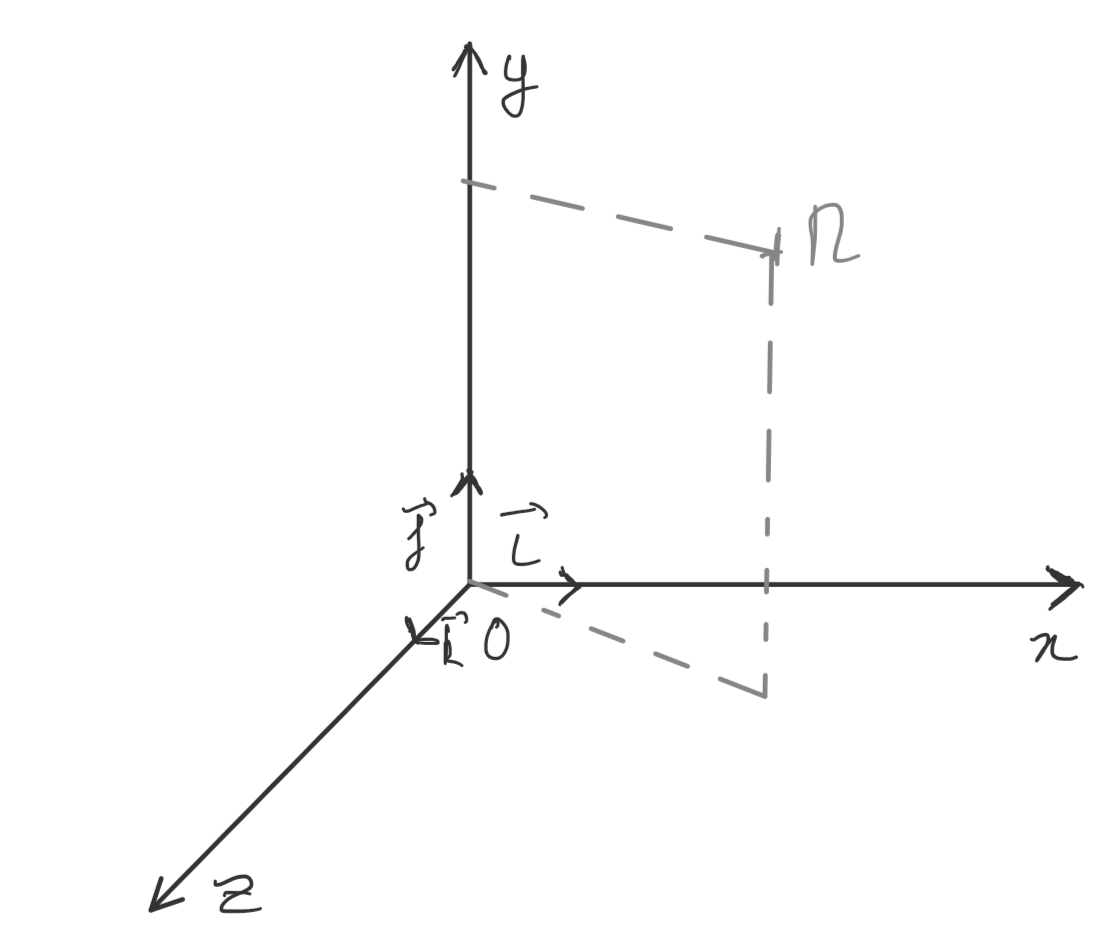
\includegraphics[width=0.5 \textwidth]{SCHEMA1-1.png}
    \caption{Schema des coordonnées cartésiennes}
    \label{fig:SCHEMA-COCA}
\end{figure}


\begin{definition}[Coordonées cartésiennes]\label{def:coordcart}
    On définit les coordonnées avce 3 vecteurs unitaires orthonormés \(\vv{i}, \vv{j}, \vv{k}\) de direction et sens indépendant du temps.
\end{definition}

\begin{corollary}[Vecteur Position]\label{col:cartpos}
    On a : \(\vv{OM} = x \vv{i} + y \vv{j}+ z\vv{k}\). \\
    D'où on a pour le déplacement élémentaire: \(d \vv{OM} = dx\vv{i}+dy\vv{j}+dz\vv{k}\) 
\end{corollary}

\begin{corollary}[Vecteur vitesse]\label{col:vitcart}
    Par définition : \(\vv{v} = \frac{d \vv{OM}}{dt}\). Or, on a \(\frac{d \vv{i}}{dt} = \frac{d\vv{j}}{dt} = \frac{d\vv{k}}{dt} = 0\).\par D'où :
    \(\vv{v} = \frac{d \vv{OM}}{dt} = \frac{dx}{dt}\vv{i} + \frac{dy}{dt}\vv{j} + \frac{dz}{dt}\vv{k} = \dot{x}\vv{i}+ \dot{y}\vv{j} + \dot{z}\vv{k}\)   
\end{corollary}
\newpage
\begin{corollary}[Vecteur accélération]\label{col:accelcart}
    On a : 
    \begin{eqnarray*}
        \vv{a} &=& \frac{d\vv{v}}{dt}\\
        &=& \frac{d^{2}\vv{v}}{dt^{2}}\\
        \vv{a} &=& \ddot{x}\vv{i} + \ddot{y}\vv{j} + \ddot{z}\vv{k}
    \end{eqnarray*}
\end{corollary}

\section{Coordonnées polaires}

\begin{figure}[!htb]
    \centering
    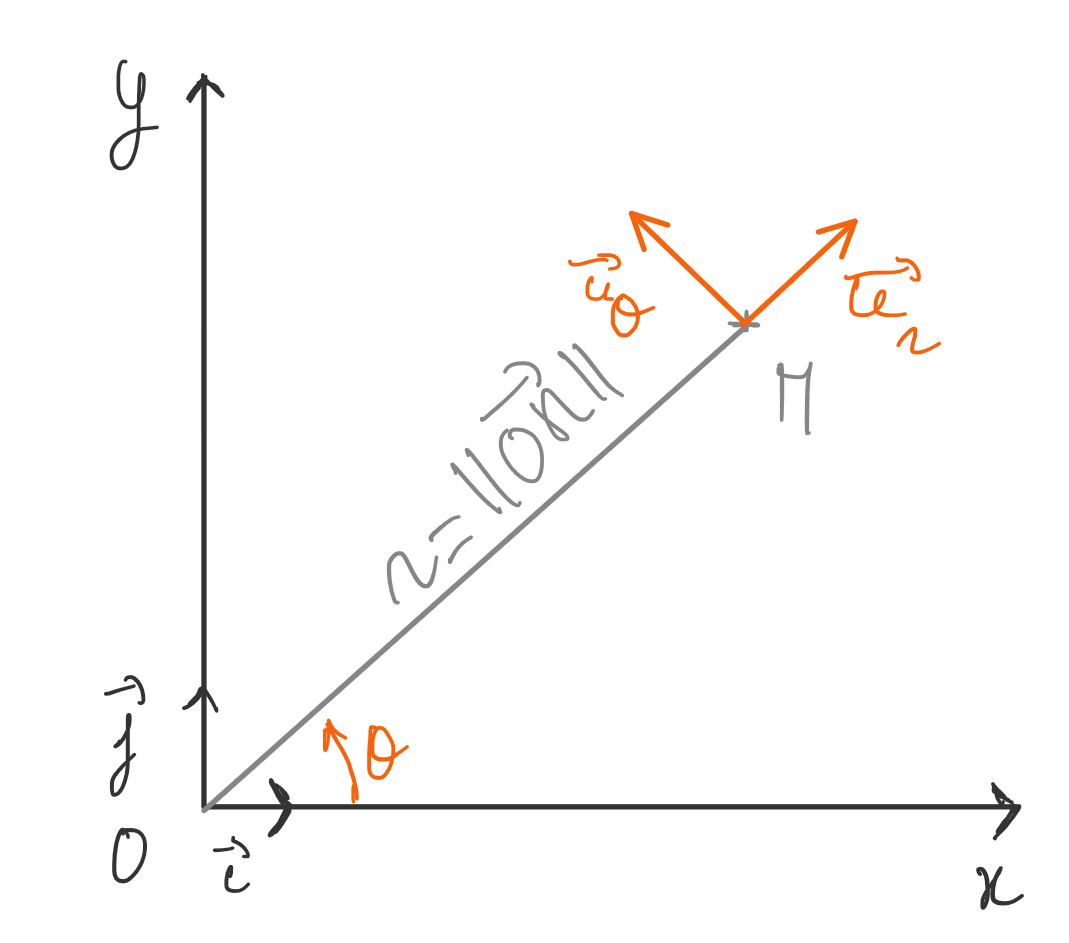
\includegraphics[width=0.5\textwidth]{SCHEMA1-2.png}
    \caption{Schema des coordonnées polaires}
    \label{fig:SCHEMA-COPOL}
\end{figure}


\begin{definition}[Coordonnées polaires]
    On définit les coordonées polaires (en 2 dimensions) avec deux vecteurs : \(\vv{u}_{r}\) et \(\vv{u}_{\theta }\). \(u_{r}\) est colinéaire au vecteur position (\(\vv{u}_{r} = \frac{\vv{OM}}{\lVert \vv{OM} \rVert }\)) et \(u_{\theta }\) est orthogonal à ce dernier, dans le même sens que l'angle orienté \((\vv{i}, \vv{OM})\).     
\end{definition}

\begin{remark}[Changement de base]
    Dans le repère d'étude, $\vv{i} \text{ et } \vv{j}$ sont constants, contrairement à $\vv{u}_\theta \text{ et } \vv{u}_r$.
On peut passer de coordonnées polaires à cartésiennes et vice-versa :
    \begin{itemize}
        \item Si on connait les coordonnées cartésiennes : \\ 
        \begin{eqnarray*}
            r = \sqrt{x^2 + y^2}\\ \cos\theta = \frac{x}{r}\\ \sin\theta = \frac{y}{r} 
        \end{eqnarray*}
        \item Si on connait les coordonnées polaires : \\
        \begin{eqnarray*}
            x = r \cos\theta\\
            y = r \sin\theta
        \end{eqnarray*}
    \end{itemize}

    \begin{corollary}[Expression des vecteurs unitaires]
        On peut donc exprimer les vecteurs unitaires \(\vv{u}_{r}\) et \(\vv{u}_{\theta }\) en fonction de \(\vv{i}\) et \(\vv{j}\) : 
        \begin{eqnarray*}
            \vv{u}_r &= \cos\theta(t) \vv{i} + \sin\theta(t)\vv{j}\\
            \vv{u}_\theta &=  -\sin\theta(t)\vv{i} + \cos\theta(t)\vv{j} 
        .\end{eqnarray*}    
    \end{corollary}
\end{remark}

\begin{corollary}[Dérivées des vecteurs unitaires]
    On dérive les vecteurs unitaires \(\vv{u}_{r}\) et \(\vv{u}_{\theta }\) en fonction du temps : 
    \begin{corollary}[\(\vec{u}_{r}\)]\label{copoldur}
        \begin{eqnarray*}
            \frac{d\vv{u}_r}{dt} &=& \frac{d}{dt} (\cos\theta(t) \vv{i} + \sin\theta(t)\vv{j})\\
            &=& \dot{\theta} (-\sin\theta) \vv{i} + \dot{\theta} \cos\theta \vv{j}\\
            &=& \dot{\theta} (-\sin\theta \vv{i} + \cos\theta \vv{j})\\
            &=& \dot{\theta}\vv{u}_\theta
        .\end{eqnarray*}
    \end{corollary} 
    
    \begin{corollary}[\(\vec{u}_{\theta}\)]\label{copoldut}
        \begin{align*}
            \frac{d\vv{u}_\theta}{dt} &= \frac{d}{dt}(-\sin\theta\vv{i}+\cos\theta\vv{j}) \\
            &= \dot{\theta}(-\cos\theta \vv{i} - \sin\theta\vv{j}) \\
            &= -\dot{\theta}\vv{u}_r
        \end{align*}
    \end{corollary}
\end{corollary}

\begin{corollary}[Vecteur position et déplacement élémentaire]\label{copolunivec}
    D'après la définition de \(\vv{u}_{r}\), on a : 
    \[
        \vv{OM} = r\vv{u}_{r} \text{ Où } r = \lVert \vv{OM} \rVert 
    \] 
    Cependant, $\vv{i} \text{ et } \vv{j}$ sont constants, contrairement à $\vv{u}_\theta \text{ et } \vv{u}_r$. Le déplacement élémentaire s'exprime alors :
    \[
        d \vv{OM} = dr\vv{u}_{r} + rd \theta \vv{u}_{\theta }
    \]
\end{corollary}

\begin{corollary}[Vecteur vitesse]\label{copolvvec}
    Le vecteur vitesse \(\vv{v}\) s'exprime : 
    \[
        \vv{v} = \dot{r}\vv{u}_{r} + r \dot{\theta }\vv{u}_{\theta}
    \] 
    \begin{explanation}
        D'après \autoref{copolunivec}, on a : \(\vv{OM} = r\vv{u}_{r}\).\par
        D'où, \(\vv{v} = \frac{d}{dt}\left[ \vv{OM} \right] = \frac{d}{dt}\left[ r\vv{u}_{r} \right] = \dot{r}\vv{u}_{r} + r\frac{d}{dt}\vv{u}_{r}\).\par
        Or, d'après \autoref{copoldur}, \(\frac{d}{dt}\vv{u}_{r} = \dot{\theta}\vv{u}_{\theta}\).\par
        D'où, \(\vv{v} = \dot{r}\vv{u}_{r} + r \dot{\theta }\vv{u}_{\theta} \,\square\) 
    \end{explanation}
\end{corollary}

\newpage

\begin{corollary}[Vecteur accélération]\label{copolavec}
    Le vecteur accélération \(\vv{a}\) s'exprime : \(\vv{a} = (\ddot{r}-r\dot{\theta}^2)\vv{u}_r + (r\ddot{\theta}+2\dot{r}\dot{\theta})\vv{u}_\theta\)  
    \begin{explanation}
        \begin{eqnarray*}
            \vv{a} &=& \frac{d}{dt}\left[ \vv{v} \right] \\
            &=&\frac{d}{dt} (\dot{r}\vv{u}_r + r\dot{\theta}\vv{u}_\theta) \\
            &=& \ddot{r} \vv{u}_r + \dot{r}\frac{d\vv{u}_r}{dt} +r\ddot{\theta}\vv{u}_\theta + r\dot{\theta}\frac{d\vv{u}_\theta}{dt}
        \end{eqnarray*}
        Or, d'après \autoref{copoldut}, \(\frac{d}{dt}\vv{u}_{\theta} = -\dot{\theta}\vv{u}_{r}\) et d'après \autoref{copoldur}, \(\frac{d}{dt}\vv{u}_{r} = \dot{\theta } \vv{u}_{\theta }\). \par
        D'où \(\vv{a}(t) = \ddot{r}\vv{u}_r +\dot{r}\dot{\theta}\vv{u}_\theta + r\ddot{\theta}\vv{u}_\theta -r\dot{\theta}\dot{\theta}\vv{u}_\theta = (\ddot{r}-r\dot{\theta}^2)\vv{u}_r + (r\ddot{\theta}+2\dot{r}\dot{\theta})\vv{u}_\theta \,\square\)  
    \end{explanation}
\end{corollary}

\begin{eg}[Cas particulier du mouvement circulaire]
    On a  : $r = R = cste $ (donc $\dot{r} = 0$). Et :  $\omega = \dot{\theta}$ (vitesse angulaire)
    D'après \autoref{copolvvec} et \autoref{copolavec}, on a : 
    \begin{eqnarray*}
        \vv{v} &=& \dot{r}\vv{u}_{r} + r\dot{\theta }\vv{u}_{\theta }\\
        \vv{a}&=&  (\ddot{r}-r\dot{\theta}^2)\vv{u}_r + (r\ddot{\theta}+2\dot{r}\dot{\theta})\vv{u}_\theta
    \end{eqnarray*}
    Or, \(\dot{r} =  0\), d'où : 
    \begin{eqnarray*}
        \vv{v} &=& R \omega \vv{u}_{\theta }\\
        \vv{a} &=& -R \omega^{2} \vv{u}_{r} + r \dot{\omega}\vv{u}_{\theta}
    \end{eqnarray*}
    Dans le cas du MCU, on a \(\dot{\omega} = 0\) : 
    \begin{eqnarray*}
        \vv{v} &=& R \omega \vv{u}_{\theta } = \text{ cste}\\
        \vv{a} &=& -R \omega^{2} \vv{u}_{r}
    \end{eqnarray*}
\end{eg}

\section{Coordonnées cylindropolaires}

\begin{figure}[!htb]
    \centering
    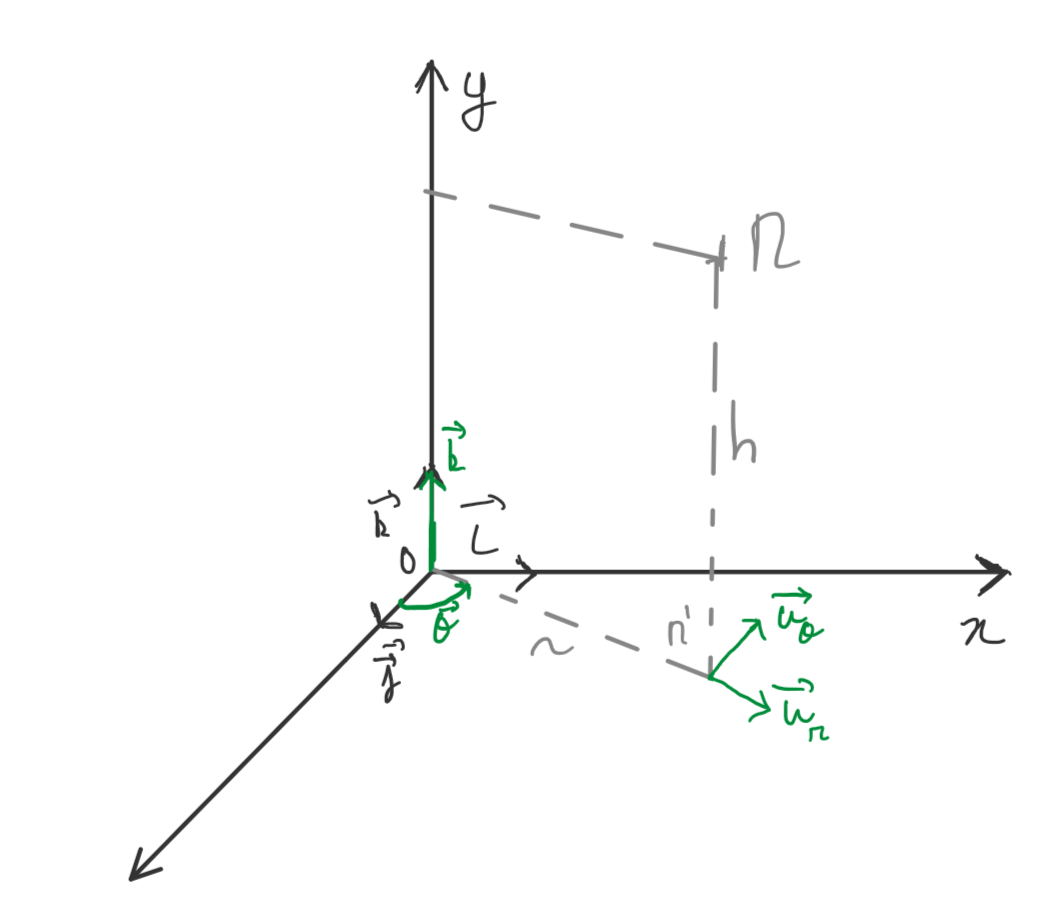
\includegraphics[width=0.5\textwidth]{SCHEMA1-3.png}
    \caption{Schema des coordonnées cylindro-polaires}
    \label{fig:SCHEMA-COCY}
\end{figure}
\newpage
\begin{definition}[Coordonnées cylindro polaires]
    On définit les coordonnées cylindro-polaires en 3 dimensions avec trois vecteurs unitaires : \(\vv{u}_{r}, \, \vv{u}_{\theta}, \text{ et }, \vv{k}\) , avec deux vecteurs en coordonnées polaires (\(\vv{u}_{r}\text{, et } \vv{u}_{\theta}\) ) et un troisième (\(\vv{k}\)), normal à ces deux, indépendant du temps, représentant la hauteur.
\end{definition}

\begin{corollary}[Vecteur position]\label{cypolpos}
    On décompose \(\vv{OM}\), en deux composantes. La première, \(MM'\) est exprimées en coordonnées polaires, alors que la deuxième, \(M'M\) est un vecteur selon le dernier vecteur unitaire, \(\vv{k}\). 
    \[
        \vv{OM} = r\vv{u}_{r} + h\vv{k}
    \] 
    Le déplacement élémentaire s'exprime alors comme-ci : 
    \[
        d \vv{OM} = dr\vv{u}_{r} + rd \theta \vv{u}_{\theta} + dh\vv{k}
    \]
\end{corollary}

\begin{corollary}[Vecteurs vitesse et accélération]\label{cycolva}
    On a le vecteur position, \autoref{cypolpos}, et les vecteurs vitesse et accélération en coordonnées cartésiennes et polaires. On utilise le fait que les composantes en coordonnées polaires et cartésiennes sont indépendantes en fonction du temps pour facilement obtenir les vecteurs position et accélération.
    \begin{eqnarray*}
        \vv{v} &=& \dot{r}\vv{u}_{r} + r \dot{\theta}\vv{u}_{\theta} + \dot{h}\vv{k}\\
        \vv{a} &=& (\ddot{r} -r \dot{\theta}^{2})\vv{u}_{r} + (\ddot{r}\theta + 2\dot{r}\dot{\theta}) + \ddot{h}\vv{k}
    \end{eqnarray*}
\end{corollary}

\section{Coordonnées sphériques}

\begin{figure}[!htb]
    \centering
    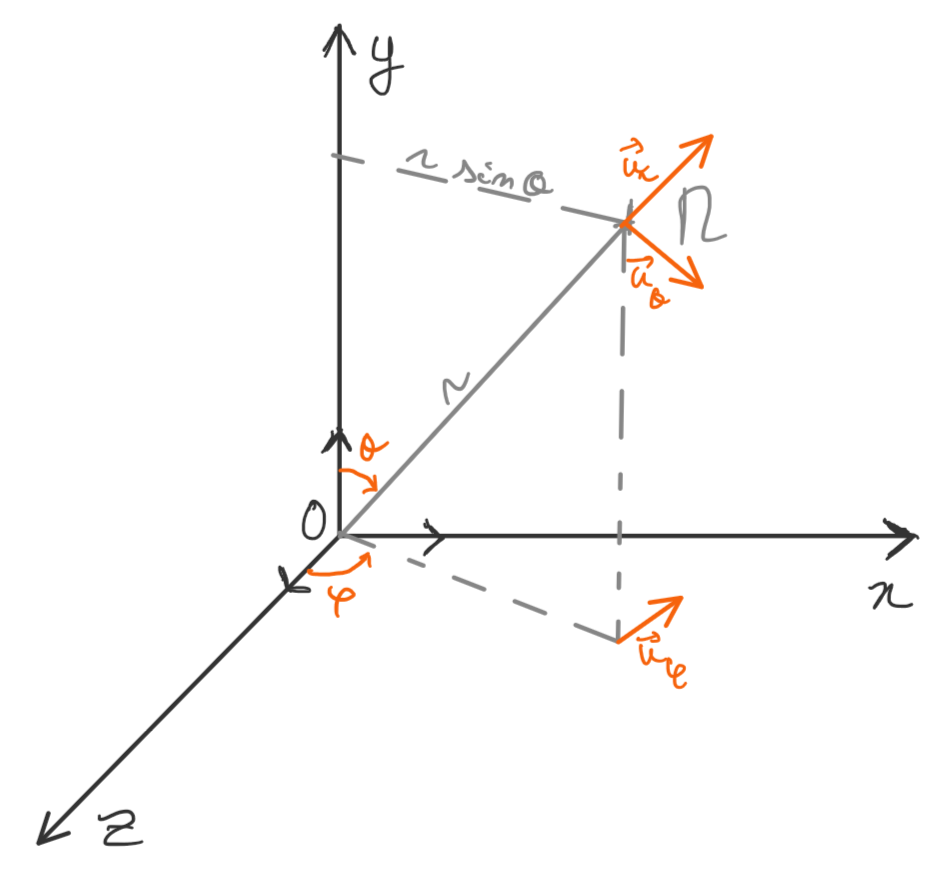
\includegraphics[width=0.4\textwidth]{SCHEMA1-4.png}
    \caption{Schema des coordonnées sphériques}
    \label{fig:SCHEMA-COSP}
\end{figure}


\begin{definition}[Coordonnées sphériques ]
    On définit les coordonnées sphériques avec 3 vecteurs, un colineaire avec la position \(\vv{u}_{r}\) , et deux représentant les angles : \(\vv{u}_{\theta}\) et \(\vv{u}_{\phi}\)  
\end{definition}

\begin{corollary}[Vecteur position]
    On a : 
    \[
        \vv{OM} = r\vv{u}_{r}
    \]
\end{corollary}

\begin{corollary}[Vecteur vitesse]
    On donne, sans preuve, le vecteur vitesse : 
    \[
        \vv{v} = \dot{r}\vv{u}_{r} + r\dot{\theta}\vv{u}_{\theta} + r\sin \theta \dot{\phi}\vv{u}_{\phi}
    \]
\end{corollary}